\documentclass{beamer}
\usepackage[utf8]{inputenc}
\usepackage{graphicx}
\usepackage{lipsum}
\usepackage{tikz}

\usetheme{Madrid}


\setbeamertemplate{footline}{
  \leavevmode%
  \hbox{%
    % Autores (ancho más grande para permitir los tres nombres completos)
    \begin{beamercolorbox}[wd=.66\paperwidth,ht=2.25ex,dp=1ex,left]{author in head/foot}%
      \usebeamerfont{author in head/foot}Luis Izquierdo Horna, Jose Zevallos Ruiz, Thurian Cevallos Vivar
    \end{beamercolorbox}%
    % Número de página
    \begin{beamercolorbox}[wd=.34\paperwidth,ht=2.25ex,dp=1ex,right]{frame number in head/foot}%
      \usebeamerfont{frame number in head/foot}\insertframenumber{} / \inserttotalframenumber
    \end{beamercolorbox}%
  }%
  \vskip0pt%
}


% Logo solo en la diapositiva de título
\titlegraphic{
  
\includegraphics[width=2.5cm]{64654f89-9b8a-47a1-9e96-0b299dc2834c.png}
}

% Datos de presentación
\title[\,]{Modelación hidrológica replicable para la evaluación de riesgos ante precipitaciones extremas en zonas vulnerables}
\author{
  \textbf{Luis Izquierdo Horna} \\
  \textbf{Jose Zevallos Ruiz} \\
  \textbf{Thurian Cevallos Vivar}
}
\institute{Universidad Tecnológica del Perú (UTP)}
\date{Mayo 2025}

\begin{document}

\begin{frame}
  \titlepage
\end{frame}

\begin{frame}{Contenido}
  \tableofcontents
\end{frame}

\section{Introducción}
\begin{frame}{Introducción}
  \small
  \begin{itemize}
    \item Las precipitaciones extremas constituyen un factor de riesgo creciente en zonas vulnerables, exacerbado por el cambio climático y la variabilidad interanual.
    \item Los modelos hidrológicos constituyen herramientas clave para la evaluación del impacto y la planificación de medidas de prevención frente a inundaciones.
    \item \textbf{Objetivo}: calibrar un modelo hidrológico replicable utilizando datos observados, completando vacíos con técnicas de inteligencia artificial, con el fin de evaluar escenarios futuros en contextos de alta incertidumbre hidrometeorológica.
  \end{itemize}
\end{frame}

\section{Metodología}
\begin{frame}{Metodología}
  \small
  \begin{itemize}
    \item El modelo se construyó con el DEM FABDEM (30 m), mapas FAO de uso y tipo de suelo, y variables meteorológicas provenientes de los productos PISCO (temperatura) y RAIN4PE (precipitación).
    \item Los caudales fueron completados usando una red neuronal LSTM, entrenada con los 7 días precedentes, evitando valores negativos mediante funciones de activación y normalización controlada.
    \item La calibración se basó en los indicadores NSE y log-NSE, con validación sobre el periodo 2000–2015 y enfoque en la representación de caudales bajos y picos extremos.
  \end{itemize}
\end{frame}

\begin{frame}{Flujo de imputación de caudales con LSTM}
  \small
  \begin{itemize}
    \item Para completar los vacíos en la serie de caudales observados, se entrenó una red LSTM con datos de caudal y precipitación de los 7 días anteriores.
    \item Se aplicó una función de activación ReLU y normalización Min-Max para asegurar que las predicciones se mantuvieran dentro del rango físico esperado.
    \item El modelo fue utilizado únicamente para completar los datos entre 2000 y 2015, manteniendo coherencia hidrológica en la calibración.
  \end{itemize}
  \vspace{0.4cm}
  \begin{center}
    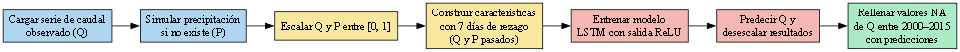
\includegraphics[width=0.95\textwidth]{flujo_lstm_qfill_300dpi.png}
  \end{center}
\end{frame}

\begin{frame}{Calibración multiobjetivo del modelo}
  \small
  \begin{itemize}
    \item Se empleó un enfoque de calibración multiobjetivo para capturar distintos aspectos del comportamiento hidrológico.
    \item Los indicadores utilizados fueron:
    \begin{itemize}
      \item \textbf{NSE} y \textbf{logNSE}: para evaluar la eficiencia general y la representación de caudales bajos.
    \end{itemize}
    \item La calibración se realizó con algoritmos evolutivos y técnicas de regionalización espacial para parámetros en zonas sin datos.
  \end{itemize}
  \vspace{0.4cm}
  % Puedes descomentar la línea siguiente cuando tengas la figura correspondiente
  % \includegraphics[width=0.9\textwidth]{nombre_figura_extraida_del_pdf.png}
\end{frame}

\begin{frame}{Parámetros calibrados en el modelo hidrológico}
  \small
  \begin{itemize}
    \item \textbf{GW\_DELAY}: Representa el retraso (en días) entre la infiltración en el perfil del suelo y su ingreso al acuífero. Valores altos indican un sistema más lento.
    \item \textbf{ALPHA\_BF}: Coeficiente de recesión del flujo base. Un valor cercano a 0 indica descarga lenta del acuífero; cercano a 1, respuesta rápida.
    \item \textbf{GWQMN}: Nivel mínimo de agua en el acuífero superficial (mm) necesario para que ocurra flujo base hacia los cauces.
    \item \textbf{RCHRG\_DP}: Fracción de recarga del acuífero profundo respecto a la recarga total del perfil del suelo.
    \item \textbf{SURLAG}: Coeficiente de retardo del escurrimiento superficial desde las HRUs hacia los cauces principales.
    \item \textbf{ESCO}: Factor de extracción de humedad por la planta, que modula la evapotranspiración según la humedad disponible.
  \end{itemize}
\end{frame}

\section{Resultados esperados}
\begin{frame}{Distribución espacial de HRUs y climatología de precipitación}
  \small
  \begin{itemize}
    \item Se muestra la delimitación de subcuencas e identificación de centroides, base para la generación de las unidades de respuesta hidrológica (HRUs).
    \item El mapa de fondo representa la climatología de precipitación anual promedio del producto RAIN4PE, que fue utilizado como forzante meteorológico en el modelo.
  \end{itemize}
  \vspace{0.1cm}
  \begin{center}
    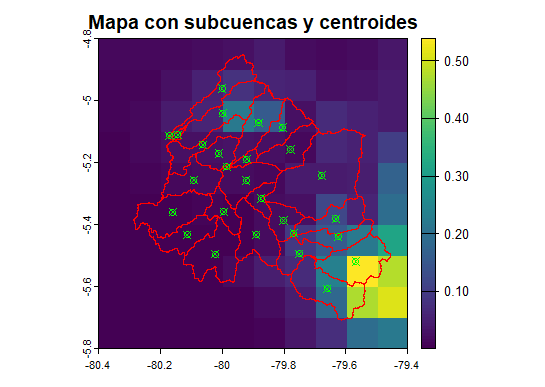
\includegraphics[width=0.60\textwidth]{centroides_clima.png}
  \end{center}
\end{frame}

\begin{frame}{Resultado de la calibración multiobjetivo}
  \small
  \begin{itemize}
    \item La figura muestra el espacio de soluciones Pareto obtenidas durante la calibración del modelo, considerando simultáneamente el indicador $1 - \log\text{NSE}$ y la métrica de forma de la curva de duración del caudal (FDCsign).
    \item Las soluciones negras corresponden al conjunto de soluciones eficientes (Pareto), mientras que en azul se resalta la \textbf{mejor solución de compromiso (BCS)}, que representa el balance óptimo entre precisión en caudales bajos y forma general del hidrograma.
    \item Esta solución fue seleccionada para evaluar los escenarios hidrológicos futuros en la cuenca de estudio.
  \end{itemize}
  \vspace{0.1cm}
  \begin{center}
    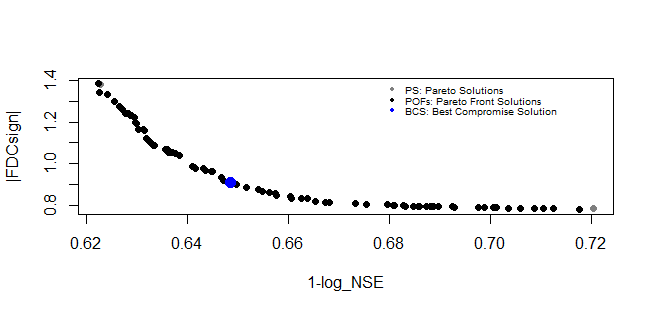
\includegraphics[width=0.65\textwidth]{Optimizacion.png}
  \end{center}
\end{frame}

\begin{frame}{Desempeño diario del modelo calibrado}
  \small
  \begin{itemize}
    \item Comparación entre caudales simulados (línea roja) y observados (puntos azules) a escala diaria, para el periodo 2000–2015.
    \item Se observan limitaciones para reproducir picos, con un NSE = 0.17 y R\textsuperscript{2} = 0.17.
    \item El modelo tiende a suavizar las crecidas rápidas, lo que sugiere oportunidad de mejora en eventos extremos.
  \end{itemize}
  \vspace{0.2cm}
  \begin{center}
    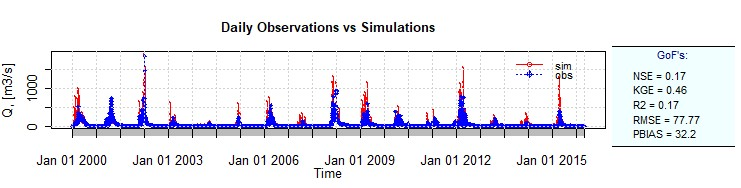
\includegraphics[width=0.85\textwidth]{calibracion_actual_diaria.png}
  \end{center}
\end{frame}

\begin{frame}{Desempeño mensual del modelo calibrado}
  \small
  \begin{itemize}
    \item A escala mensual, el modelo muestra una mejor representación de la dinámica hidrológica acumulada.
    \item Se obtiene un NSE = 0.77 y R\textsuperscript{2} = 0.77, lo que refleja una buena capacidad para simular estacionalidad y volúmenes mensuales.
    \item Este nivel de ajuste resulta adecuado para estudios de tendencia y escenarios climáticos.
  \end{itemize}
  \vspace{0.2cm}
  \begin{center}
    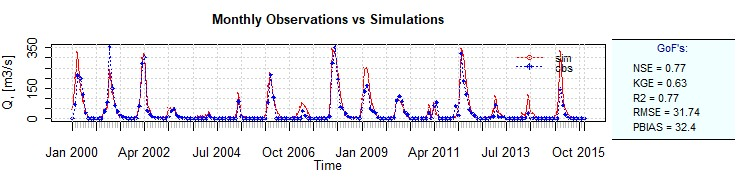
\includegraphics[width=0.85\textwidth]{calibracion_actual_mensual.png}
  \end{center}
\end{frame}


\section{Conclusiones}
\begin{frame}{Conclusiones}
  \small
  \begin{itemize}
    \item La replicabilidad del enfoque RAIN4PE permite su aplicación en otras regiones con escasa información, especialmente en zonas de montaña y cuencas transfronterizas.
    \item El uso de caudales para ajustar la precipitación mejora el cierre del balance hídrico y la confiabilidad del modelado.
    \item Se promueve una gestión del riesgo hidrológico basada en evidencia empírica y en escenarios climáticos más realistas.
    \item RAIN4PE puede adoptarse como referencia oficial para evaluar otros productos de precipitación en Perú y Ecuador.
  \end{itemize}
\end{frame}


\begin{frame}{Gracias}
  \centering
  \Large ¿Preguntas?
\end{frame}

\end{document}
